\chapter{Forecasting}
\label{app:forecasting}

% % NEW
%   \subsection{Foundation-Model Forecasting Configurations}
%   \label{app:foundation-configurations}

%   \begin{table}[htbp]
%   \centering
%   \footnotesize
%   \renewcommand{\arraystretch}{1.15}
%   \begin{tabularx}{\textwidth}{
%   >{\raggedright\arraybackslash}p{0.19\textwidth}
%   >{\raggedright\arraybackslash}X
%   >{\raggedright\arraybackslash}X}
%   \toprule
%   Setting & TabPFN & TabICLv2 \\
%   \midrule

%   Implementation &
%   \texttt{tabpfn} 8.0.8; generic
%   \texttt{tabpfn-v2-regressor.ckpt} &
%   \texttt{tabicl} 2.1.1; default TabICLv2 regression weights \\

%   Estimator &
%   \texttt{TabPFNRegressor}, eight estimators, seed 137 &
%   \texttt{TabICLRegressor}, eight estimators, seed 42 \\

%   Training scope &
%   Pooled across T2, T4 and T9, with tower indicators &
%   Pooled across T2, T4 and T9, with tower indicators \\

%   Predictors &
%   The 57 predictors listed in Table~\ref{tab:fc_tabpfn_features} &
%   The same 57-predictor frame \\

%   Target observations &
%   QC-valid pre-origin \texttt{y\_observed} only &
%   QC-valid pre-origin \texttt{y\_observed} only \\

%   Missing predictors &
%   Training-set mean imputation &
%   Training-set mean imputation \\

%   Context &
%   Equal-weight combination of an all-history spike-corrected model,
%   a 1,095-day model and a 1,460-day model &
%   Most recent 1,460 days \\

%   Target processing &
%   Raw target for the all-history and 1,095-day components; tower-wise
%   median/IQR normalisation for the 1,460-day component &
%   Tower-wise median/IQR normalisation \\

%   Point estimate &
%   Predictive median &
%   Predictive median \\

%   Final prediction &
%   Arithmetic mean of the three component forecasts &
%   Single-model prediction; exploratory ensembles were not retained \\

%   \bottomrule
%   \end{tabularx}
%   \caption{Implementation settings for the B18 tabular-foundation-model
%   forecasting experiments. All preprocessing statistics and event thresholds
%   were estimated from pre-origin training data only.}
%   \label{tab:app_foundation_configurations}
%   \end{table}

\begin{figure}[htbp]
\centering
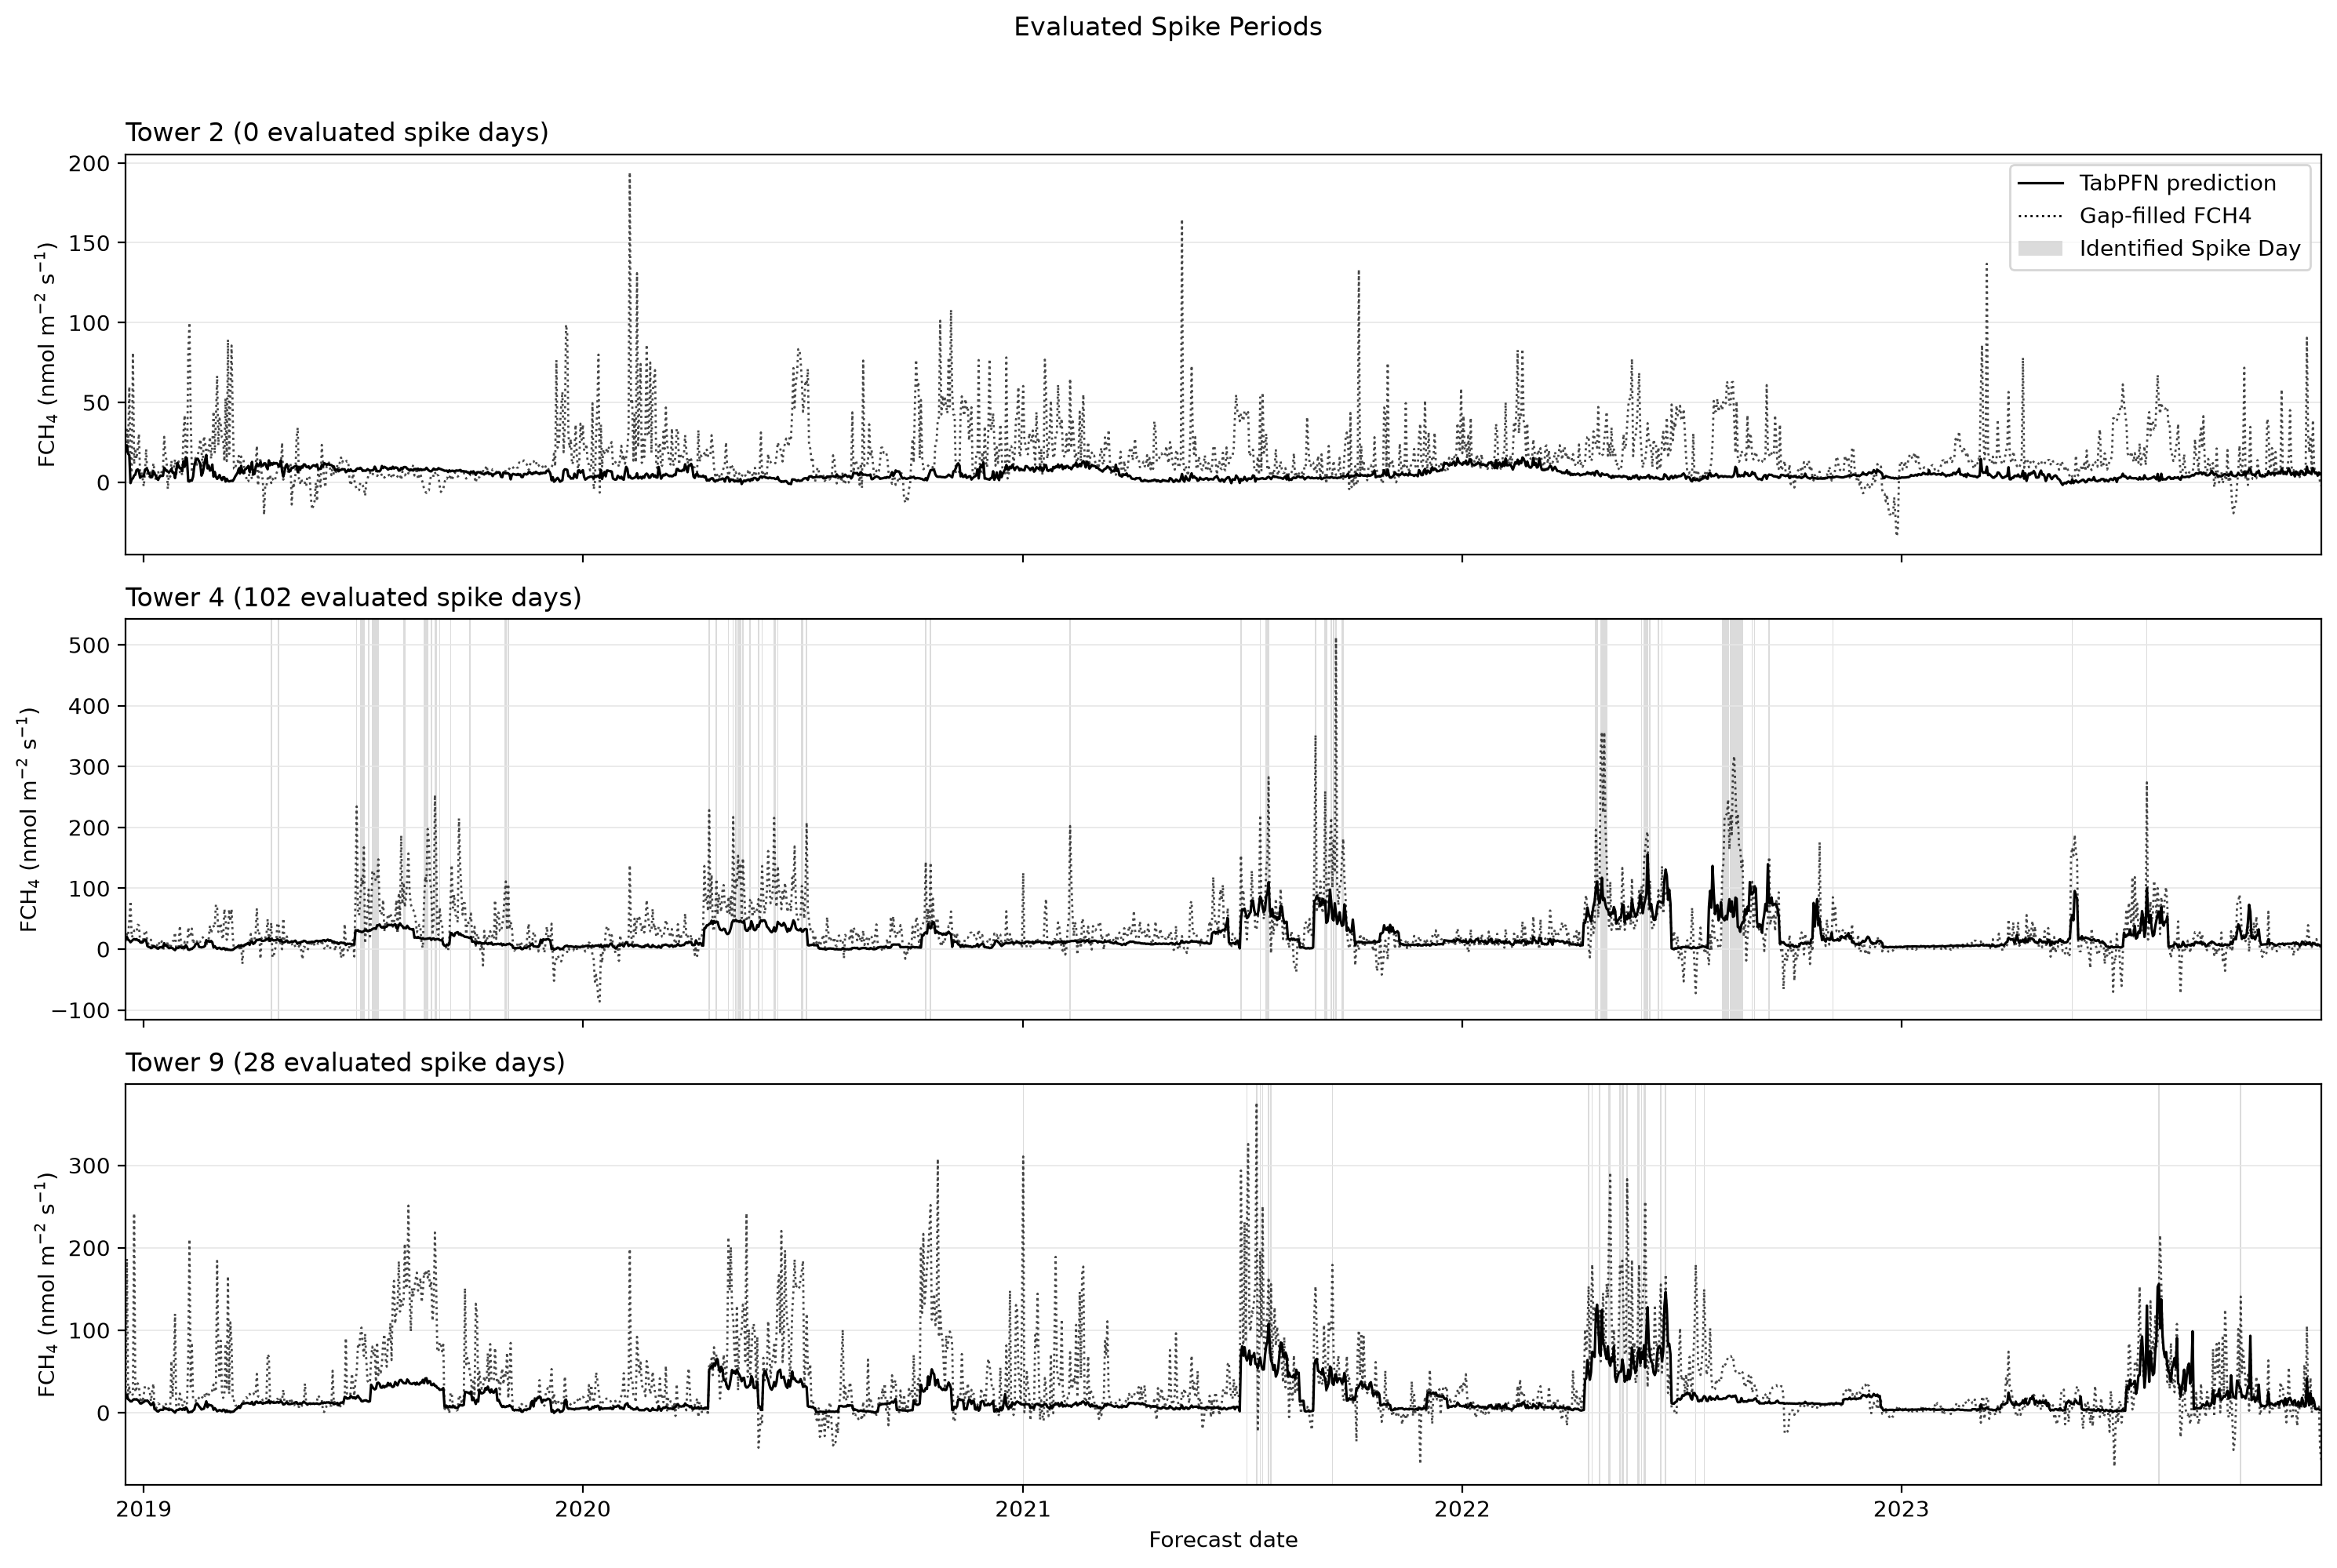
\includegraphics[width=\textwidth]{Figures/ch5_B18_p95_spike_timing_all_towers.png}
\caption{Temporal distribution of the spike observations used in the
forecasting evaluation. Grey bands mark QC-valid observations above the
tower- and origin-specific pre-forecast 95th-percentile threshold; the solid
line shows the TabPFN prediction and the dotted line
shows the gap-filled FCH\textsubscript{4} series for context. The evaluated
sample contains no spike days at T2, 102 at T4 and 28 at T9.}
\label{fig:app_fc_spike_timing}
\end{figure}

\begin{figure}[htbp]
\centering
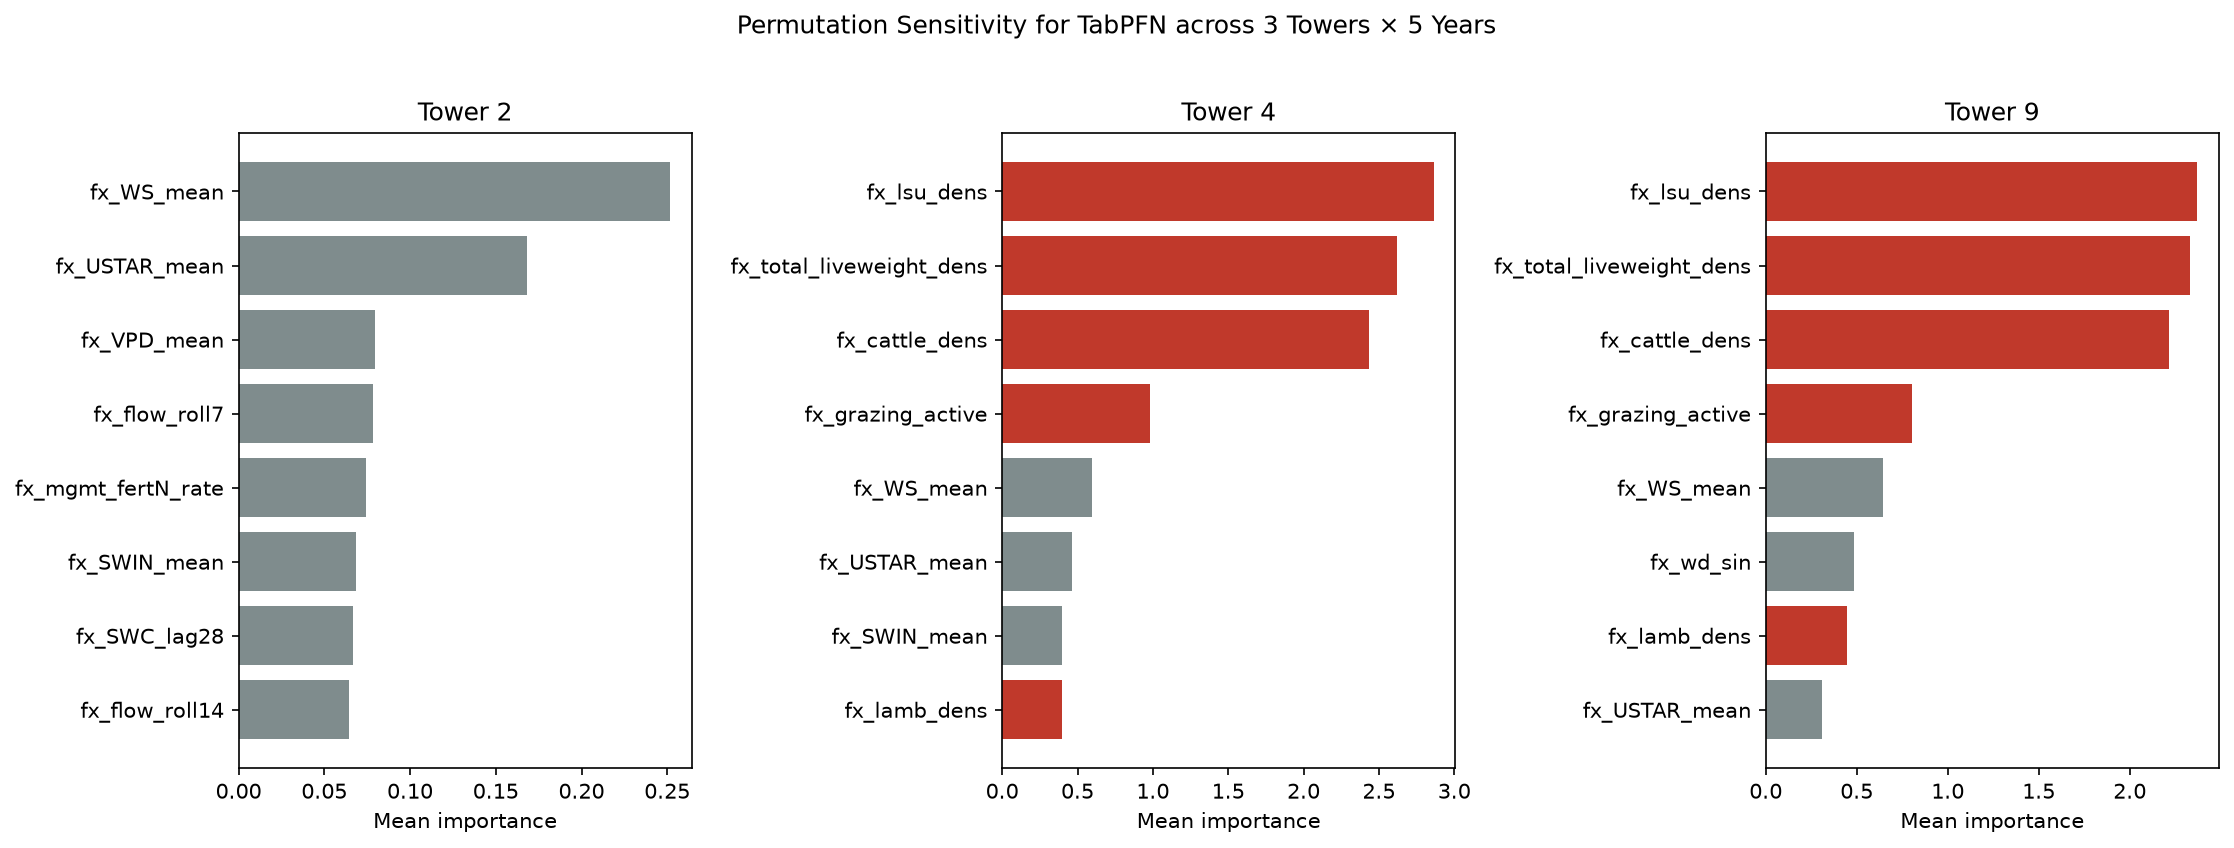
\includegraphics[width=\textwidth]{Figures/ch5_tabpfn_permutation_sensitivity_by_tower.png}
\caption{Tower-specific permutation-sensitivity rankings for the TabPFN
model. The figure shows the leading predictors
within T2, T4 and T9, complementing the pooled ranking in
Figure~\ref{fig:fc_tabpfn_importance}.}
\label{fig:app_fc_importance_by_tower}
\end{figure}

\begin{figure}[htbp]
\centering
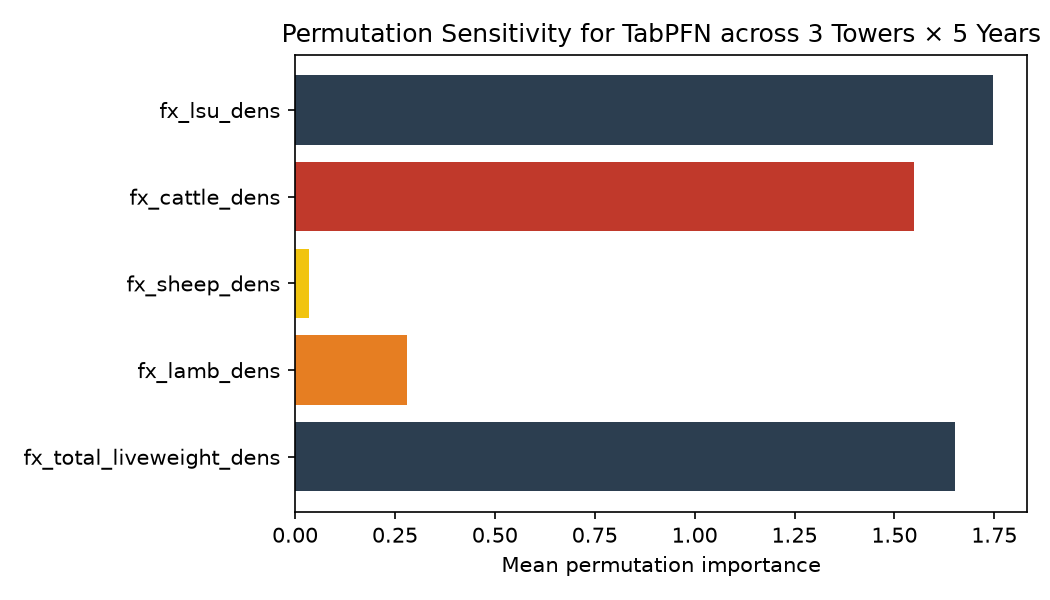
\includegraphics[width=0.75\textwidth]{Figures/ch5_tabpfn_permutation_sensitivity_species.png}
\caption{Permutation sensitivity of the livestock-species predictors in the
TabPFN model. The comparison separates the
contributions of cattle, sheep and lamb density within the broader livestock
signal.}
\label{fig:app_fc_importance_species}
\end{figure}

\begin{figure}[htbp]
\centering
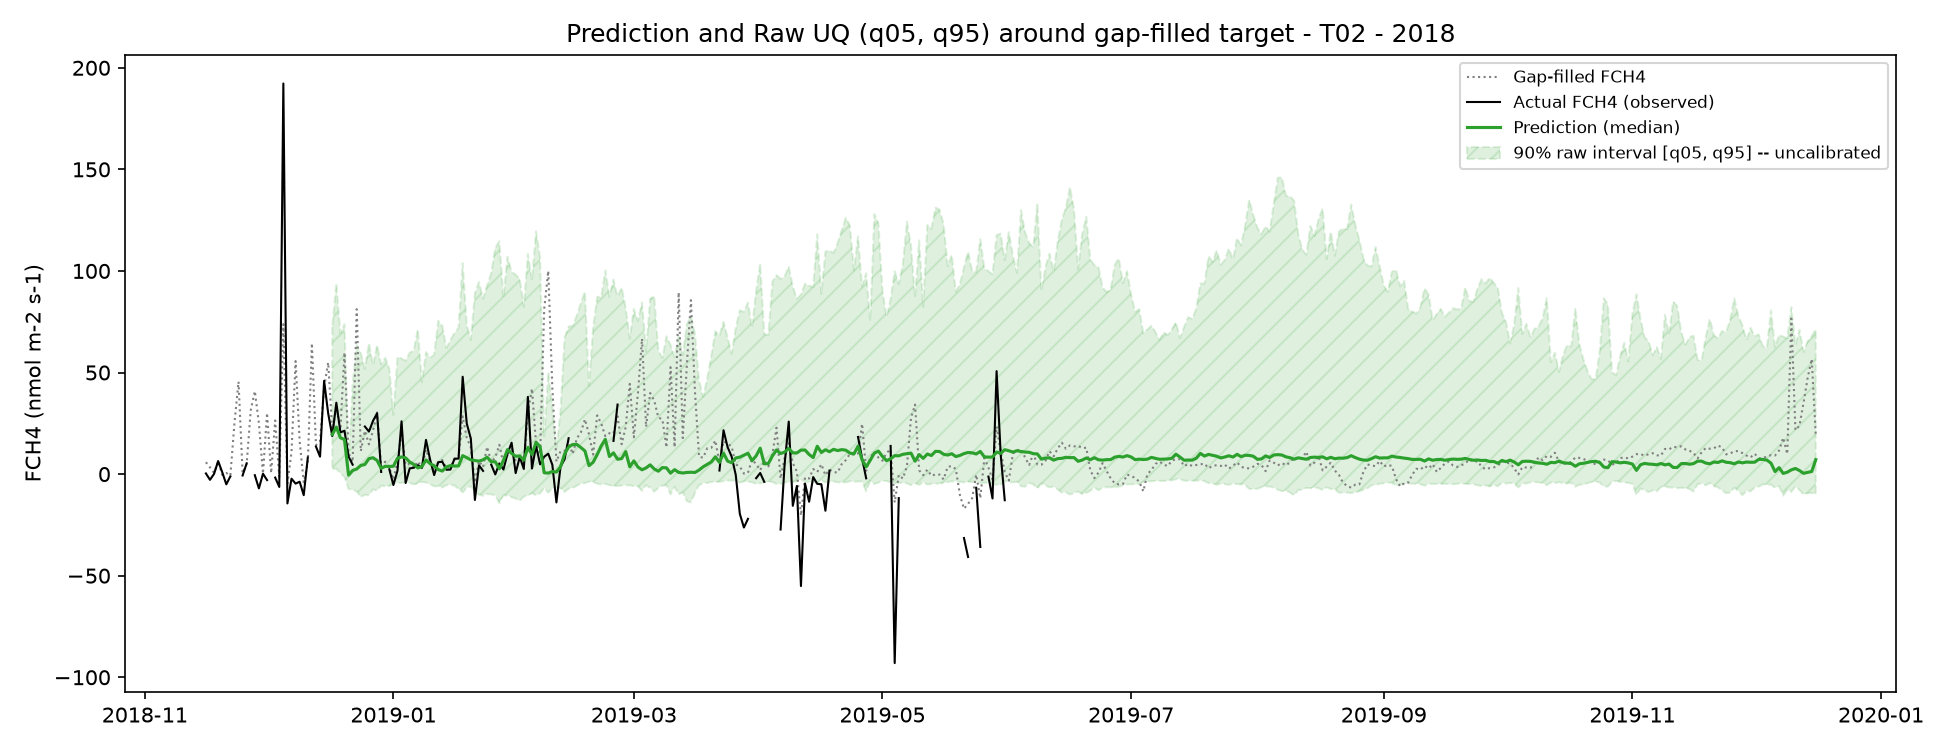
\includegraphics[width=\textwidth]{Figures/cqr_gallery/ch5_cqr_forecast_T02_2018.png}
\caption{Representative 365-day TabPFN forecast at T2 from the 2018 forecast
origin. The green line is the median forecast, the black line shows available
observations, and the dotted line provides the gap-filled series as context.
The hatched region is the native raw 90\% quantile interval. Conformal
calibration was not applied because the available T2 observations were
insufficient to construct a leave-one-origin-out calibration set.}
\label{fig:app_fc_uq_t2_raw}
\end{figure}

\begin{figure}[htbp]
\centering
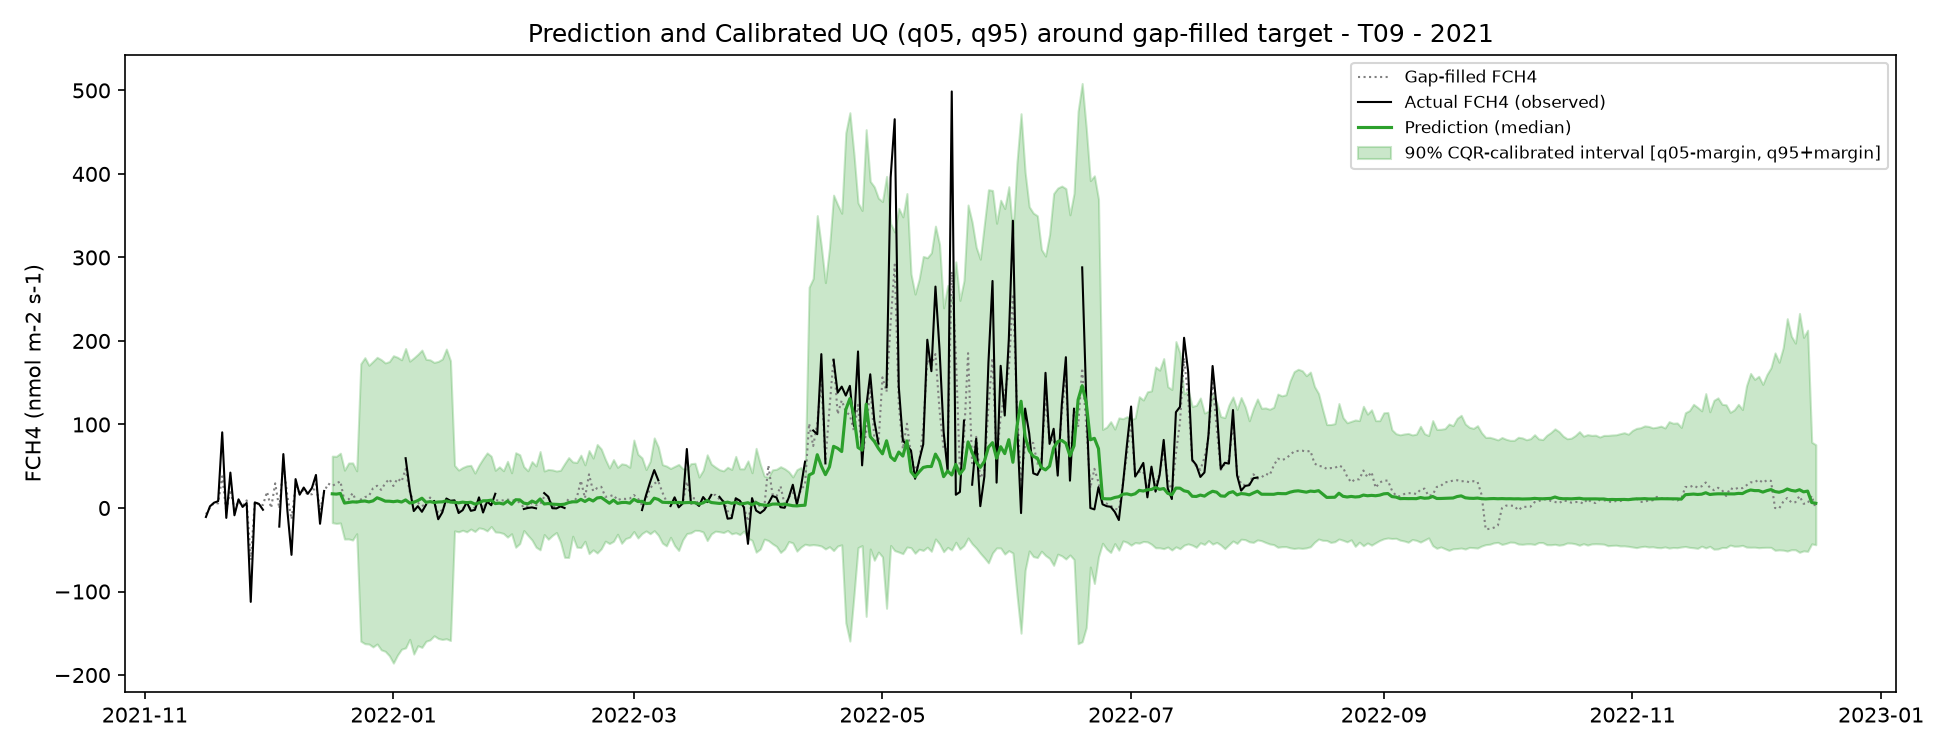
\includegraphics[width=\textwidth]{Figures/cqr_gallery/ch5_cqr_forecast_T09_2021.png}
\caption{Representative 365-day TabPFN forecast at T9 from the 2021 forecast
origin. The green line is the median forecast, the black line shows available
observations, the dotted line provides the gap-filled series as context, and
the shaded region is the 90\% CQR-calibrated prediction interval across the
complete forecast horizon.}
\label{fig:app_fc_cqr_t9}
\end{figure}

\FloatBarrier

